\documentclass[../thesis.tex]{subfiles}

\begin{document}

\section*{Εντοπισμός ακατάλληλου περιεχομένου μέσω μηχανικής όρασης}
Όπως αναφέραμε, ένα μέρος της εφαρμογής αφορά στο ανέβασμα εικόνων από τους χρήστες για εμφάνιση στο δημόσιο προφίλ τους.
Ήταν σημαντικό να προσφέρουμε τη δυνατότητα αυτή στους χρήστες, καθώς θεωρήσαμε ότι οι φωτογραφίες καθιστούν την εφαρμογή πιο εύχρηστη, επιτρέποντας στους χρήστες να αναγνωρίσουν εύκολα ο ένας τον άλλον, ενώ ενισχύουν ταυτόχρονα την κοινωνική διάσταση της εφαρμογής.
Ωστόσο, αυτή η επιλογή που δίνεται στους χρήστες ενδέχεται να παρουσιάσει κινδύνους.
Ο κάθε χρήστης μπορεί να ανεβάσει φωτογραφίες ακατάλληλου περιεχομένου, και οι φωτογραφίες αυτές μπορεί να εμφανιστούν στις συσκευές άλλων χρηστών, γεγονός που πρέπει σε κάθε περίπτωση να αποφευχθεί.
Η επώνυμη φύση της εφαρμογής που επιβάλλεται από την απαίτηση ταυτοποίησης μειώνει σημαντικά την πιθανότητα τέτοιων περιστατικών, όμως πρέπει να είμαστε σε θέση να εντοπίσουμε άμεσα αυτό το υλικό αν αυτό εμφανιστεί.

Για τον σκοπό αυτό χρησιμοποιήσαμε ένα μοντέλο μηχανικής μάθησης.
Αφού δοκιμάσαμε αρκετά μοντέλα, αποφασίσαμε να επιλέξουμε για την περίπτωσή μας το OpenNSFW2\cite{Yung_Open-NSFW_2_2023}, το οποίο αποτελεί σύγχρονη υλοποίηση του διάσημου μοντέλου OpenNSFW\cite{Mahadeokar_Pesavento_2016} της Yahoo.
Το μοντέλο είναι τύπου Residual Network, και βασίζεται στο ResNet50 της Microsoft, με υλοποίηση στη βιβλιοθήκη Tensorflow.
Επιλέξαμε το συγκεκριμένο μοντέλο καθώς έπειτα από δοκιμές συμπεράναμε ότι προσφέρει τη μεγαλύτερη ακρίβεια με μικρό κόστος τόσο όσον αφορά το μέγεθος όσο και τον υπολογιστικό φόρτο.
Για τη λειτουργία του μοντέλου δημιουργήσαμε μέσω του framework Flask έναν απλό τοπικό server Python\footnote{Αρχικά επιχειρήσαμε να χρησιμοποιήσουμε το Node.js και για αυτόν τον σκοπό ώστε να έχουμε ομοιομορφία όσον αφορά τη γλώσσα, όμως κάποιες ασυνέπειες στην υλοποίηση των διεπαφών του Tensorflow έκαναν αδύνατη τη φόρτωση του μοντέλου στη JavaScript} ο οποίος λειτουργεί παράλληλα με τον κύριο server.
Ο server αυτός φορτώνει το μοντέλο μηχανικής όρασης και αναμένει αιτήματα HTTP για την αξιολόγηση του περιεχομένου ενός δεδομένου αρχείου.
Μόλις λάβει ένα αίτημα, ο server φορτώνει το αρχείο εικόνας στο μοντέλο, και λαμβάνει ως αποτέλεσμα την πιθανότητα εμφάνισης ακατάλληλου περιεχομένου, την οποία στέλνει ως απόκριση πίσω στον κύριο server.
Είναι σημαντικό να σημειωθεί ότι εφόσον οι δύο servers ανήκουν σε διαφορετικές διεργασίες η λειτουργία τους είναι παράλληλη, και καθώς η επικοινωνία επιτυγχάνεται μέσω ασύγχρονων non-blocking HTTP calls ο κύριος server σε καμία περίπτωση δεν παύει να επεξεργάζεται αιτήματα περιμένοντας την απόκριση του server μηχανικής όρασης.
Έτσι μπορούμε να έχουμε γρήγορη αναγνώριση εικόνων και επομένως άμεση εντόπιση πιθανών παραβάσεων, χωρίς όμως αυτό να είναι εις βάρος της ταχύτητας του server και επομένως της εμπειρίας του χρήστη.

\section*{Authentication}
Για την ταυτοποίηση των χρηστών είναι απαραίτητη η επικοινωνία της εφαρμογής με το σύστημα ταυτοποίησης του Πολυτεχνείου, το οποίο βασίζεται στο πρωτόκολλο SAML\footnote{Το SAML (Security Assertion Markup Language) είναι ένα σύστημα σχεδιασμένο για την ασφαλή ανταλλαγή ισχυρισμών (assertions) που αφορούν την ταυτότητα και τις εξουσιοδοτήσεις ενός χρήστη}.
Αντί να επικοινωνούμε απευθείας με τον Identity Provider της σχολής, εκτελούμε την ταυτοποίηση μέσω ενός server Keycloak\footnote{Ο server Keycloak δημιουργήθηκε από τους φοιτητές της σχολής ... } ο οποίος είναι ρυθμισμένος έτσι ώστε να λειτουργεί ως Identity Broker εκ μέρους του.
\todo{Find out who to credit for Keycloak server}
Χρησιμοποιώντας το Keycloak η ταυτοποίηση μπορεί να γίνει μέσω του πρωτοκόλλου OpenID Connect το οποίο είναι πιο εύκολα υλοποιήσιμο από το SAML σε μοντέρνες εφαρμογές.

\subsection*{OAuth και OpenID Connect}
Ο όρος authentication αφορά την ταυτοποίηση ενός χρήστη, ενώ το authorization αφορά μόνο την παροχή άδειας σε μία υπηρεσία για την πρόσβαση σε προστατευμένους πόρους εκ μέρους του χρήστη.
Οι δύο έννοιες είναι στενά συνδεδεμένες, ωστόσο είναι σημαντικό να μη συγχέονται.
Οι προδιαγραφές του OAuth 2.0 δημοσιεύθηκαν τον Οκτώβριο του 2012 από τον οργανισμό IETF (Internet Engineering Task Force) ως επικαιροποίηση των προδιαγραφών του πρωτοκόλλου OAuth 1.0 που είχε δημοσιευθεί το 2007, και γρήγορα υιοθετήθηκαν από πολλές υπηρεσίες του διαδικτύου.
Παρά το γεγονός ότι το OAuth αποτελεί αυστηρά πρωτόκολλο authorization και δεν είναι σχεδιασμένο για authentication, από την απαρχή του το OAuth χρησιμοποιήθηκε καταχρηστικά για το authentication χρηστών από μεγάλο μέρος του διαδικτύου.
Αυτή η λανθασμένη χρήση του OAuth για authentication παρουσιάζει κινδύνους για την ασφάλεια των δεδομένων του χρήστη\cite{oauth_net}.

Το OpenID Connect (OIDC) είναι ένα πρωτόκολλο σχεδιασμένο ειδικά για ασφαλή authentication χρηστών.
Δημοσιεύτηκε το 2014 ως βελτίωση του παλαιότερου πρωτοκόλλου OpenID 1.0/2.0, και βασίζεται πάνω στο authorization framework του OAuth 2.0.
Το OIDC παρουσιάζει μία μέθοδο ταυτοποίησης η οποία είναι συμβατή με το ήδη εδραιωμένο πρωτόκολλο OAuth 2.0, επιτρέποντας την εύκολη υλοποίηση του authentication τόσο από πλευράς του Identity Provider όσο και από πλευράς του Client\cite{oidc_faq}.

\begin{figure}[!ht]
    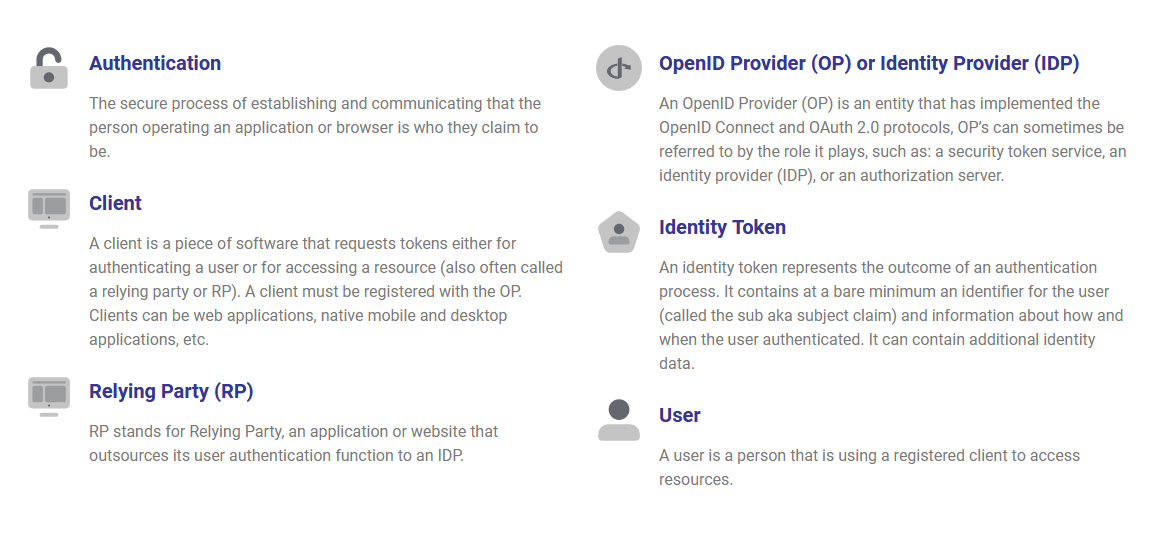
\includegraphics[width=\textwidth]{oidc_definitions.png}
    \centering
    \caption{Ορισμοί των βασικών όρων που χρησιμοποιούνται στο πρωτόκολλο OpenID Connect\cite{oidc_faq}.}
\end{figure}

Θα περιγράψουμε συνοπτικά τη διαδικασία ταυτοποίησης που γίνεται για την πρόσβαση των στοιχείων του χρήστη από την ιστοσελίδα της εφαρμογής μέσω του browser.
Η ροή ταυτοποίησης ξεκινάει όταν ο χρήστης ζητήσει πρόσβαση στον πόρο που απαιτεί δικαιώματα πρόσβασης, δηλαδή στη σελίδα του προφίλ του.
Ο web server δέχεται το αίτημα και ελέγχει αν ο συγκεκριμένος χρήστης είναι ήδη συνδεδεμένος.
Αν όχι, τότε ξεκινάει το λεγόμενο authorization code flow που ορίζεται από το πρωτόκολλο OpenID Connect για την ταυτοποίηση του χρήστη.
Ο server (Relying Party) ανακατευθύνει τον browser του χρήστη στην ιστοσελίδα του Keycloak (Identity Provider) με τις κατάλληλες παραμέτρους που προσδιορίζουν το αίτημα (client ID/secret, redirect URI, code challenge κ.ά.).
Αφού ο χρήστης εισάγει τα στοιχεία του, το Keycloak ανακατευθύνει με τη σειρά του τον browser πίσω στην ιστοσελίδα του server, περιλαμβάνοντας στις παραμέτρους του συνδέσμου έναν κώδικα που δίνει πρόσβαση στα στοιχεία του χρήστη.
Μόλις ο server λάβει την αίτηση αυτή από τον χρήστη, παρουσιάζει τον κώδικα στο Keycloak, το οποίο τελικά του προσφέρει τα στοιχεία του χρήστη με τη μορφή JWT.
Σε αυτό το σημείο ο server επαληθεύει την εγκυρότητα του token, και αφού εξάγει τις πληροφορίες που χρειάζεται (στην περίπτωσή μας τον ΑΜ και ονοματεπώνυμο) τις αποθηκεύει στο session του χρήστη.
Από το σημείο αυτό και πέρα, κάθε αίτημα του χρήστη προς τον server συνοδεύεται από ένα session cookie το οποίο ο server μπορεί να χρησιμοποιήσει για να αντιστοιχίσει το αίτημα του χρήστη με το κατάλληλο session, και επομένως με την ταυτότητα του.

\begin{figure}[!ht]
    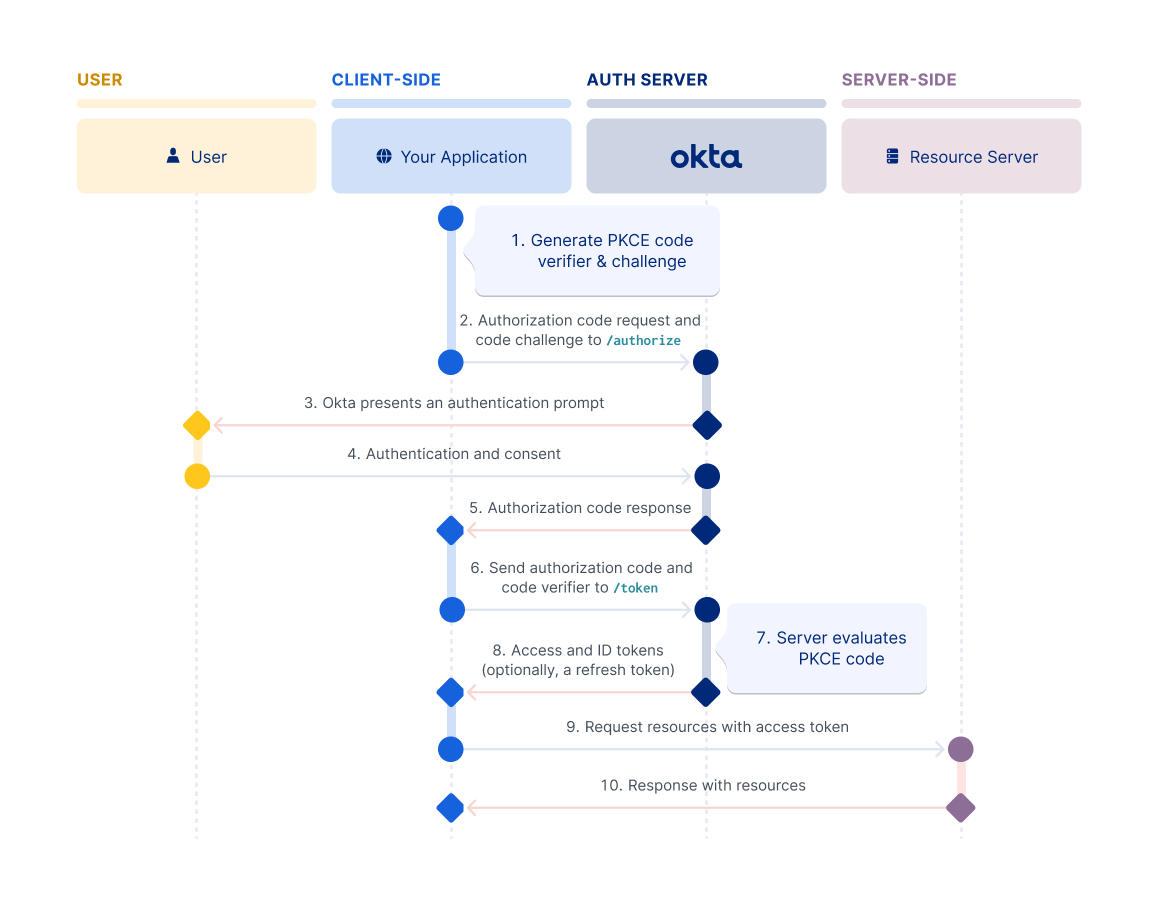
\includegraphics[width=\textwidth]{oauth_code_flow}
    \centering
    \caption{Το authorization code flow σε περισσότερη λεπτομέρεια. Στην περίπτωσή μας ο \textit{client} είναι ο server, και ο \textit{auth server} είναι το Keycloak. H διαδικασία σταματάει στο βήμα 8 καθώς μας ενδιαφέρει μόνο το ID Token το οποίο ταυτοποιεί τον χρήστη, και δε χρειαζόμαστε το access token για πρόσβαση σε εξωτερικό API/\textit{resource server}\cite{okta_code_flow}.}
\end{figure}

Το authentication του χρήστη στην εφαρμογή κινητού λειτουργεί με παρόμοιο τρόπο, με τη διαφορά ότι ο \textit{client} είναι πια εφαρμογή κινητού και όχι browser, γεγονός που σημαίνει ότι απαιτείται ειδική μέριμνα για την προστασία των προσωπικών στοιχείων του χρήστη.
Για τον σκοπό αυτό συστήνεται η χρήση του AppAuth, μίας βιβλιοθήκης που δημιουργήθηκε από την OpenID Foundation για authentication εντός κινητών εφαρμογών.
Το βασικό σημείο που χρήζει προσοχής είναι η επικινδυνότητα της χρήσης \textit{embedded user-agent} και συγκεκριμένα των in-app webviews στη διαδικασία ταυτοποίησης.
Τα webviews χρησιμοποιούνται εκτεταμένα σε κινητές εφαρμογές καθώς επιτρέπουν τη φόρτωση ιστοσελίδων εντός της εφαρμογής, παρέχοντας αυξημένο έλεγχο στην εμφάνιση και στη λειτουργία του "browser".
Αυτές όμως οι δυνατότητες που προσφέρουν τα webviews τα καθιστούν πλέον ακατάλληλα για authentication, καθώς η εφαρμογή έχει πλήρη πρόσβαση στα στοιχεία σύνδεσης που ο χρήστης εισάγει στη φόρμα ταυτοποίησης.\cite[\S8.12]{rfc8252}
Για αυτόν τον λόγο το AppAuth χρησιμοποιεί εξ ολοκλήρου τον αξιόπιστο default system browser του χρήστη\footnote{Safari στις συσκευές iOS, και Google Chrome στις συσκευές Android} για το authentication flow, επιστρέφοντας στο τέλος της διαδικασίας μόνο το authorization code στην εφαρμογή.
Έτσι προστατευόμαστε από πιθανούς κινδύνους ασφαλείας που εγκυμονούν τα webviews, και διατηρείται η εμπιστοσύνη του χρήστη στην ασφάλεια της εφαρμογής.
Τέλος, ο εξωτερικός browser διατηρεί όλους τους αποθηκευμένους κωδικούς και τα sessions του χρήστη, διευκολύνοντας τη σύνδεση του στην εφαρμογή και επομένως βελτιώνοντας την εμπειρία του.

\end{document}